\section{Preliminary Study}

% TODO: This paragraph does not actually explain anything about the schemas used in the study

To demonstrate the effectiveness and domain extensibility of \mrstudyr, we studied the mutants of the nine schemas in
Table~\ref{tbl:study-schemas} with the presented tool. Similar to the studies of Wong and
Mathur~\cite{mathur1994empirical}, \mr~performed mutant sampling with $x$ value increments larger than $1\%$.
Specifically, for this experiment, \mr~analysed $x$ at $1\%$ and $10\%$, then increased by $10\%$ intervals to a maximum
value of $90\%$. By setting the granularity of the experiment to $10\%$ intervals, \mr~reduces the cost of performing
retrospective analysis, while confirming trends from prior work, as shown in Figure~\ref{fig:graph}.

% These schemas were chosen due to the range in triviality --- the total number of constraints ({\small$\sum$Constraints}).

% CJM: to find the distance between original and reduced mutation scores
% this example below is just for an x value of 1 and for random sampling

% d <- read_data("sqlite-avmdefaults.dat")
% d <- select_empirical_study_schemas(d)
% d <- select_normal_data(d)
% t <- analyse(d)
% t_filt <- dplyr::filter(t, method == "random_sampling", percentage == 1)
% diff <- abs((t_filt$original_mutation_score - t_filt$reduced_mutation_score))
% max(diff)
% [1] 0.4666667

% CJM: to find the min and max RMSE at a given percentage
% this example below is just for an x value of 1 and for random sampling

% d <- read_data("sqlite-avmdefaults.dat")
% d <- select_empirical_study_schemas(d)
% d <- select_normal_data(d)
% t <- analyse(d)
% t_filt <- dplyr::filter(t, method == "random_sampling", percentage == 1)
% c <- analyse_calculations(t_filt)
% max(c$root_mean_squared_error)
% [1] 0.20367
% min(c$root_mean_squared_error)
% [1] 0.06175125

% CJM: to create the visualisation currently in the paper:

% d <- read_data("sqlite-avmdefaults.dat")
% d <- select_empirical_study_schemas(d)
% d <- select_normal_data(d)
% t <- analyse(d)
% pers <- c(1, 10, 20, 40)
% t_filt <- dplyr::filter(t, method == "random_sampling", percentage %in% pers)
% visualise_mutation_score_across_schemas(t_filt)

% TODO: Right now, this paragraph does not explain the meaning of the symbols in the boxplot

% Introduce the boxplot and then give a quick overview of the results

Figure~\ref{fig:graph} is a box-and-whisker plot with the schemas on the horizontal-axis and the mutation scores of the
reduced sets after random sampling at the $x$ values of 1\%, 10\%, 20\%, and 40\% on the vertical-axis.  We chose these
$x$ values because they serve to confirm a previously observed trend of mutation score accuracy improving as $x$
increased. Moving from top-left to bottom-right, the boxes in Figure~\ref{fig:graph} show this improvement in accuracy
by becoming smaller as $x$ increases.

% Explain why there is the increase in the scores and then analyse the results according to T_b and RMSE

% TODO: This content does not contain any results about Kendall's T_b correlation! This needs to be added soon.

This increase in accuracy occurs because the mutation scores of reduced sets with smaller fractional thresholds are
often very volatile and can thus vary largely based on one or a few mutants; in contrast, the mutation scores of sets
with higher fractional thresholds are substantially more stable. In the top-left of Figure~\ref{fig:graph}, $x$ is
evaluated at 1\%.  In this quadrant of Figure~\ref{fig:graph}, sets' mutation scores are as distant from the original
mutation as $0.467$.  Additionally, at this threshold, the ``lower-is-better'' metric, RMSE, ranges from $0.062$ to
$0.204$.  Stability is demonstrated in mutation scores of sets with as small as a 10\% maximum fractional threshold,
with RMSE ranging from $0.013$ to $0.065$.  At this same threshold, Wong and Mathur observed that mutation scores of
reduced sets were within $0.16$ of the original set's mutation score~\cite{mathur1994empirical}. Using \mr~to
retrospectively perform random sampling with an $x$ value of 10\%, we observed mutation scores of reduced sets to be
within $0.13$ of the original set's mutation score.

% TODO: Be consistent in the use of the phrases that describe the variable x. Some of this may be too wordy.

The trend of the mutation score becoming more accurate as the maximum fractional threshold increases remains true for
$x$ values of 20\% and 40\%. At the thresholds of 20\% and 40\%, the mutation scores of reduced sets are within $0.083$
and $0.075$ of the original mutation scores, respectively. While it is possible that these results may be specific to
the domain of schemas, we note that future studies can easily be conducted as \mr~is available for download from
GitHub~\cite{tool}.

% sample data used or database schemas being the domain analysed.

\begin{figure}[!t]

  \centering
  \hspace*{-1em}

  \begin{minipage}{4in}
    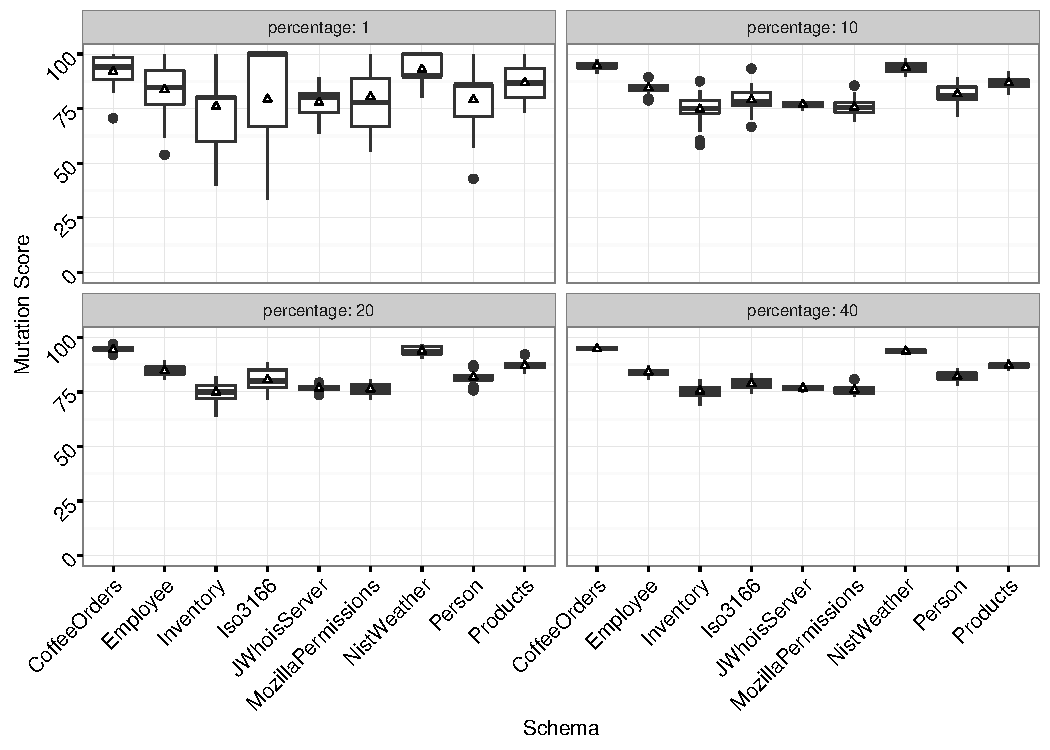
\includegraphics[scale = 0.5]{graphs/schema_vs_ms.pdf}
  \end{minipage}

  \caption{\label{fig:graph}Graph displaying mutation scores for database schemas.}

  \vspace{-1.8em}

\end{figure}

